\documentclass[a4paper, 12pt, oneside]{scrbook}

\usepackage[ngerman]{babel}		
\usepackage[onehalfspacing]{setspace}  %Zeilenabstand 1.5
\PassOptionsToPackage{hyphens}{url}\usepackage[hidelinks]{hyperref}

\usepackage[backend=biber,style=numeric,sorting=none]{biblatex}
\usepackage[T1]{fontenc}	  	
\usepackage[utf8]{inputenc}
\usepackage{acronym}
\usepackage[left=2.5cm,right=2.5cm,top=2.5cm,bottom=2.5cm,includeheadfoot]{geometry} % 2.5cm Randabstand werden als Minimum von der DHBW vorgeschrieben
\usepackage{graphicx}
\usepackage{epstopdf}
\usepackage{float}
\usepackage{booktabs}
\usepackage{caption}
\usepackage{csquotes}
\usepackage{fancyhdr}
\usepackage{wrapfig}
\usepackage{scrhack}

\usepackage{blindtext}
\usepackage[parfill]{parskip} % Entfernt Einrückung zu Beginn eines Paragraphen

\renewcommand*{\headfont}{\normalfont}
\renewcommand*{\multicitedelim}{\addsemicolon\space}
\renewcommand*{\headrulewidth}{0pt}
\renewcommand*{\arraystretch}{1.5}

\setlength{\parskip}{1.5ex}

\usepackage{comment}

% Code Formatierung
\usepackage{listings}
\usepackage{color}

\renewcommand{\lstlistingname}{Codebeispiel}
\renewcommand{\lstlistlistingname}{Codebeispielverzeichnis}

\definecolor{dkgreen}{rgb}{0,0.6,0}
\definecolor{gray}{rgb}{0.5,0.5,0.5}
\definecolor{mauve}{rgb}{0.58,0,0.82}

\lstset{frame=tb,
	language=Java,
	morekeywords={typeof, new, true, false, catch, function, return, null, catch, switch, var, if, in, while, do, else, case, break},
	ndkeywords={class, export, boolean, throw, implements, import, this, await, async},
	aboveskip=3mm,
	belowskip=3mm,
	showstringspaces=false,
	columns=flexible,
	basicstyle={\small\ttfamily},
	numbers=none,
	numberstyle=\tiny\color{gray},
	keywordstyle=\color{blue},
	commentstyle=\color{dkgreen},
	stringstyle=\color{mauve},
	breaklines=true,
	tabsize=3,
	captionpos=b
}

\bibliography{bibliography.bib}
\begin{document}

\frontmatter

% Hierin müssen Matrikelnummer Name usw. gesetzt werden.
\def\doctype{Dokumententyp}
\def\title{Entwicklung von Web-Front-Ends mit Vue.js}
\def\author{Lars Rickert}

\begin{titlepage}

	\vspace{10mm}

	\begin{center}
		\vspace{5mm}

		\huge \title

		\vspace{14.2pt}

		%\large \doctype


		\vspace{42.6pt}

		\large Studienarbeit T3\_3101

		\vspace{42.6pt}

		\small des Studienganges Angewandte Informatik an der \\
		\large Dualen Hochschule Baden-Württemberg Mosbach

		\vspace{14.2pt}

		
\includegraphics[height=1.5cm]{prefix/image/logo-dhbw.pdf}

		\vspace{42.6pt}

		\small von \\
		\large \author
	\end{center}

	\vspace{140pt}

	\begin{table}[h]
		\centering
		\begin{tabular}{ll}
			% \small Bearbeitungszeitraum            & XXX Wochen     \\
			\small Matrikelnummer, Kurs            & 2858031, INF19B \\
			\small Gutachter der Dualen Hochschule & Philipp Abele   \\
		\end{tabular}
	\end{table}

	\vspace{49.7pt}

	\fancypagestyle{empty}{
		\fancyhf{}
		\fancyfoot[C]{\today}
	}

\end{titlepage}


\pagenumbering{gobble}
\vspace*{100pt}

\begin{center}
	Eigenständigkeitserklärung
\end{center}

\textit{
	\noindent Ich versichere hiermit, dass ich meine Studienarbeit mit dem Thema: \\
	\glqq\title\grqq{} \\
	selbstständig verfasst und keine anderen als die angegebenen Quellen und Hilfsmittel benutzt habe. \\
	Ich versichere zudem, dass die eingereichte elektronische Fassung mit der gedruckten Fassung übereinstimmt.}

\vspace*{4em}

\hrulefill \\
Ort, Datum \hspace{8em} Unterschrift

\newpage


\addchap*{Abstract}

\subsection*{Deutsche Version}

Deutscher Abstract

\newpage

\subsection*{English version}

English Abstract

\tableofcontents

% Abbildungsverzeichnis
\cleardoublepage
\phantomsection
\addcontentsline{toc}{chapter}{\listfigurename}
\pagenumbering{Roman}
\listoffigures

% Tabellenverzeichnis
\cleardoublepage
\phantomsection
\addcontentsline{toc}{chapter}{\listtablename}
\listoftables

%Codebeispiel Verzeichnis
\cleardoublepage
\phantomsection
\addcontentsline{toc}{chapter}{\lstlistlistingname}
\lstlistoflistings

% Abkürzungsverzeichnis (siehe Ordner "content")
\chapter{Abkürzungsverzeichnis}
\begin{acronym}
	\acro{SFC}{Single-File Component}
	\acroplural{SFC}[SFCs]{Single-File Components}
	\acro{CMS}{Content Management System}
\end{acronym}


\mainmatter

%%%%%% Inhalt (siehe Ordner "content") %%%%%%
\input{content/einleitung.tex}
\chapter{Technologien}

%
% TypeScript
%
\section{TypeScript}
\label{sec:typescript}

TypeScript ist eine Programmiersprache von Microsoft, die JavaScript um ein Typensystem erweitert. So können u.A. Fehler frühzeitig (während der Entwicklung) erkannt und behoben sowie Autovervollständigungen geboten werden. TypeScript-Code kann nicht direkt ausgeführt werden, sondern muss vorher zu JavaScript transpiliert werden. Jeder gültige JavaScript-Code ist dadurch auch gültiger TypeScript-Code \cites[vgl.][]{TypeScript}[vgl.][]{TypeScriptForJSDevelopers}.

Abbildung \ref{fig:typescript} zeigt einen TypeScript-Code, bei dem der Parameter der Funktion als Array typisiert wurde. Wird nun z.B. eine ungültige Methode, wie \lstinline{trim} aufgerufen, gibt TypeScript eine Fehlermeldung aus, da Arrays diese Methode nicht besitzen.

\begin{figure}[H]
  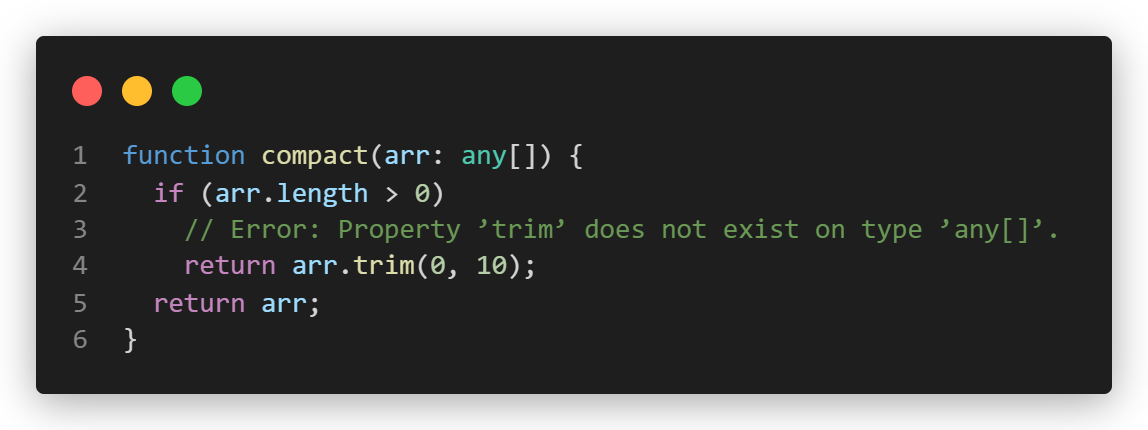
\includegraphics[width=0.9\textwidth]{images/typescript-example.png}
  \centering
  \caption[Beispiel für TypeScript-Code]{Beispiel für TypeScript-Code}
  \label{fig:typescript}
\end{figure}

Bestehende JavaScript-Projekte können inkrementell auf TypeScript umgestellt werden, indem TypeScript vorerst nur als Typ-Überprüfung verwendet wird. Dabei können Kommentare in den vorhandenen JavaScript-Code eingefügt werden, wodurch TypeScript anschließend den Code überprüfen kann (siehe Abildung \ref{fig:typescript-js}) \cite[vgl.][]{TypeScript}. Da hierbei anders als in Abbildung \ref{fig:typescript} kein TypeScript-Code eingefügt wird, muss der Code nicht transpiliert werden, bietet jedoch auch nicht den vollen Funktionsumfang von TypeScript.

\begin{figure}[H]
  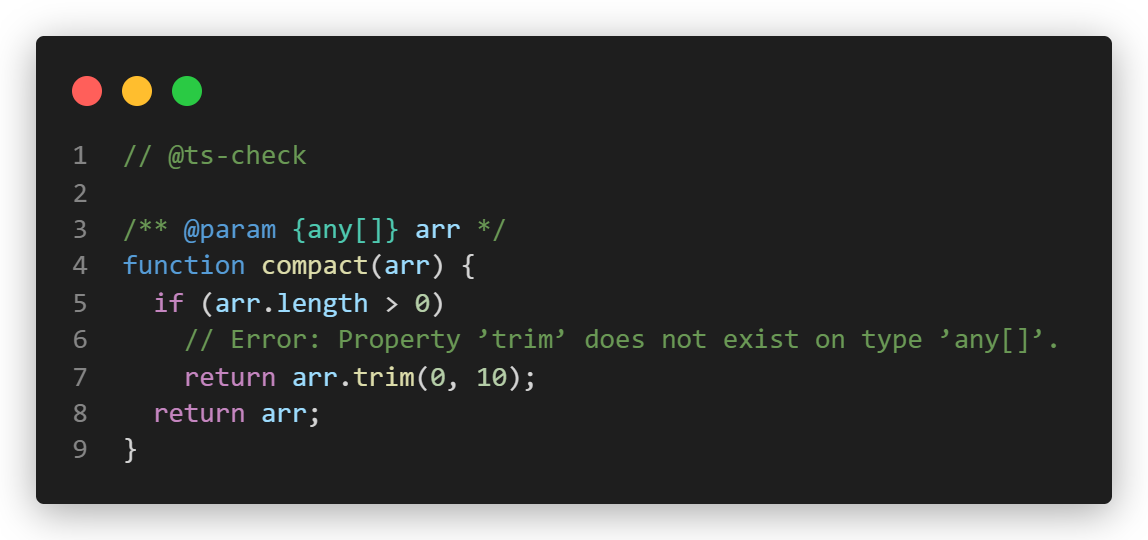
\includegraphics[width=0.9\textwidth]{images/typescript-example-js.png}
  \centering
  \caption[Erweiterung von JavaScript-Code um TypeScript Typ-Überprüfung]{Erweiterung von JavaScript-Code um TypeScript Typ-Überprüfung}
  \label{fig:typescript-js}
\end{figure}

%
% Sass
%
\section{Sass}
\label{sec:sass}
Sass ist eine Stylesheet-Sprache, die zu CSS kompiliert wird. Sie vereinfacht die Verwendung von CSS, indem weitere Funktionen, wie z.B. Verschachtlung, bereitgestellt werden. Dabei ist sie vollständig zu CSS kompatibel, d.h. jeder CSS-Code ist gültiger Sass-Code \cite[vgl.][]{SassDocs}. Die erweiterten Funktionen helfen dabei robusten und wartbaren CSS-Code zu schreiben \cite[vgl.][]{SassDocs}.

Abbildung \ref{fig:store-definition} zeigt einen Vergleich desselben Codes in CSS und Sass. Durch Sass kann hierbei redundanter Code verhindert werden. Für Interessierte sei für weitere Funktionen auf \cite{SassGuide} verwiesen.

\begin{figure}[!htb]
  \begin{minipage}{0.48\textwidth}
    \centering
    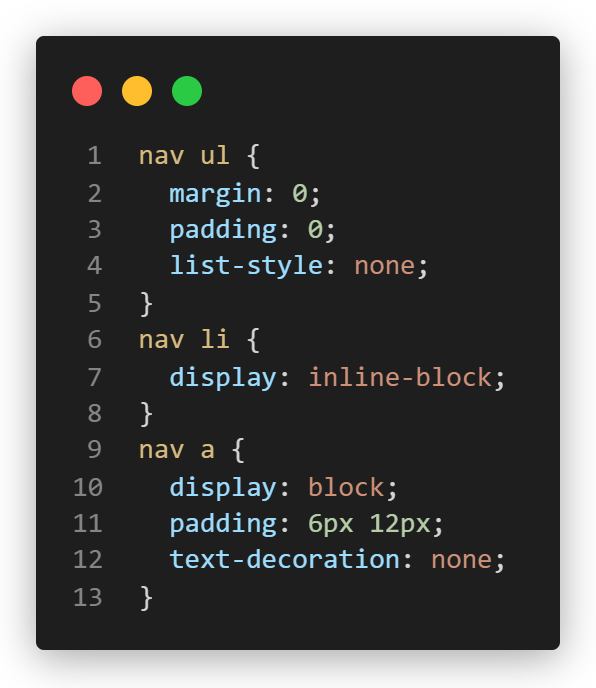
\includegraphics[width=.95\linewidth]{images/css-example.png}
  \end{minipage}\hfill
  \begin{minipage}{0.48\textwidth}
    \centering
    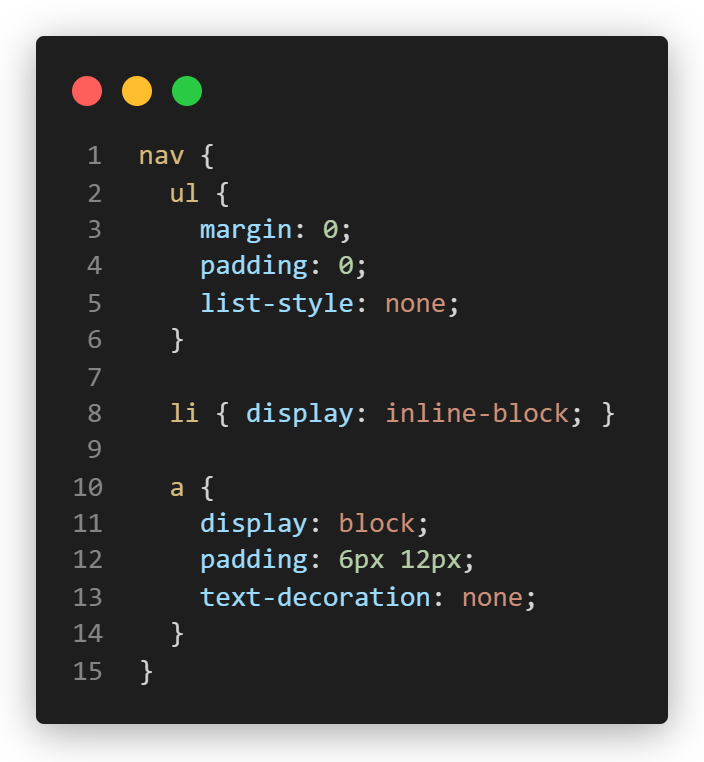
\includegraphics[width=1\linewidth]{images/sass-example.png}
  \end{minipage}
  \caption[Vergleich von CSS und Sass]{Vergleich von CSS (links) und Sass (rechts) am Beispiel von Verschachtlung \cite{SassGuide}}
  \label{fig:store-definition}
\end{figure}

%
% Vue
%
\section{Vue}

Für die Erstellung der Benutzeroberfläche (im Folgenden \glqq Frontend\grqq{} genannt) wird Vue verwendet. Vue ist ein progressives JavaScript-Framework, das die Frontend-Entwicklung vereinfachen soll. Progressiv bedeutet hierbei, das es für das gesamte Frontend oder auch nur für Teile dessen verwendet werden kann. Vue kann folglich mit anderen Technologien verwendet oder Schritt-für-Schritt (progressiv) in bereits vorhandene Projekte integriert werden \cite[vgl.][]{VueIntroduction}.

%
% Vue - Grundlagen von Komponenten
%
\subsection{Grundlagen von Komponenten}
\begin{figure}[H]
  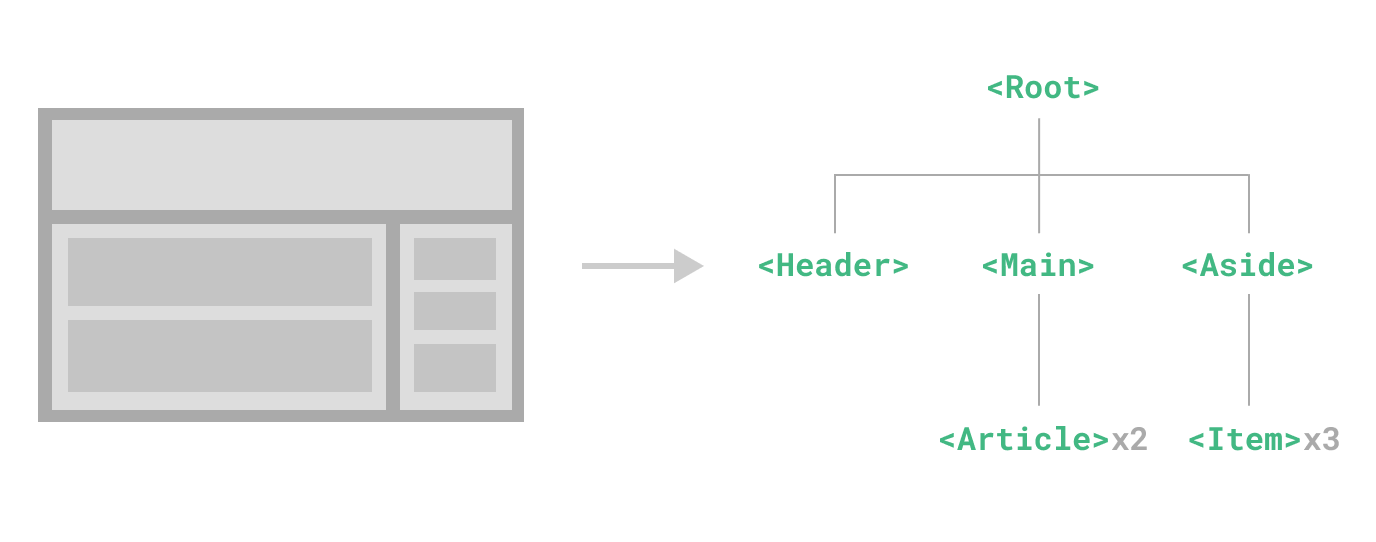
\includegraphics[width=0.9\textwidth]{images/vue-components.png}
  \centering
  \caption[Vue-Komponenten]{Strukturierung des Frontends durch Vue-Komponenten \cite{VueComponentBasics}}
  \label{fig:vue-components}
\end{figure}

Vue-Komponenten erlauben die Unterteilung des Frontends in unabhängige, isolierte und wiederverwendbare Teile. So wird das Frontend in kleinere Komponenten gegliedert (siehe Abbildung \ref{fig:vue-components}), die dann die benötigte Logik kapseln und unabhängig entwickelt werden können \cite[vgl.][]{VueComponentBasics}.

Vue bietet mehrere Möglichkeiten, um eine Komponente zu definieren. Im Rahmen dieser Studienarbeit werden sogenannte \aclu{SFC} (\acs{SFC}) verwendet (siehe Abbildung \ref{fig:vue-example}). Jede Komponente wird hierbei in einer Datei mit der Dateiendung \lstinline{.vue} definiert. Nachdem die Komponente in einer anderen Datei importiert wurde, kann sie wie ein herkömmliches HTML-Element verwendet werden (siehe Abbildung \ref{fig:vue-example-usage}) \cite[vgl.][]{VueComponentBasics}.

\begin{figure}[!htb]
  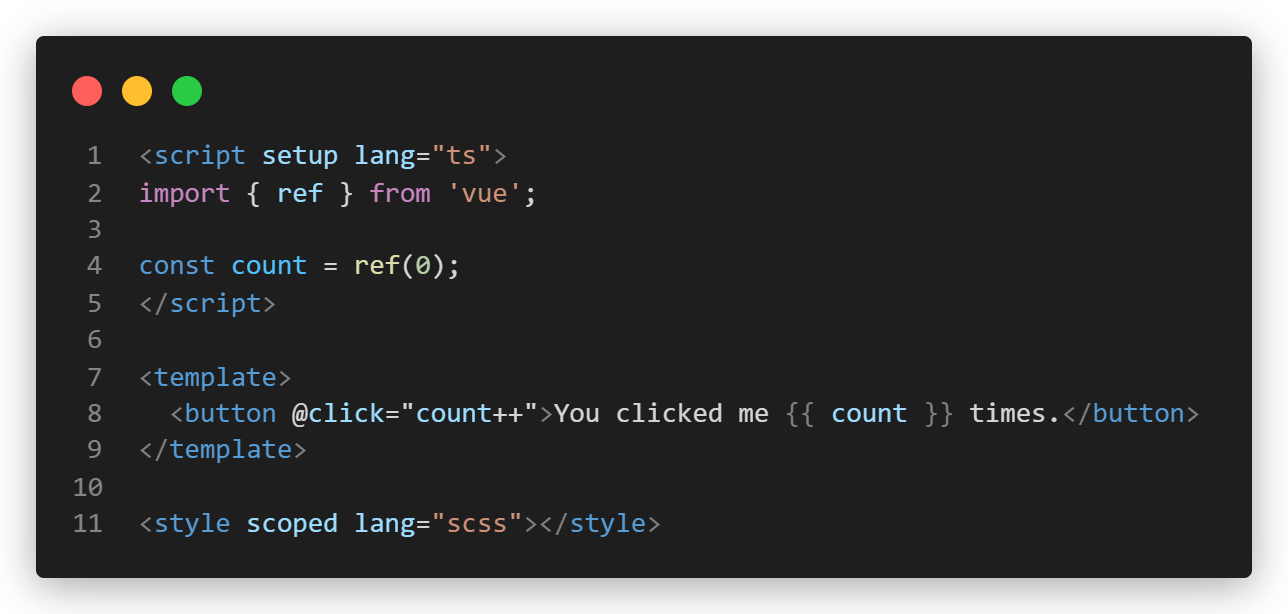
\includegraphics[width=0.9\textwidth]{images/vue-example.png}
  \centering
  \caption[Beispiel einer Vue-Komponente]{Beispiel einer Vue \ac{SFC} \cite{VueComponentBasics}}
  \label{fig:vue-example}
\end{figure}

\begin{figure}[!htb]
  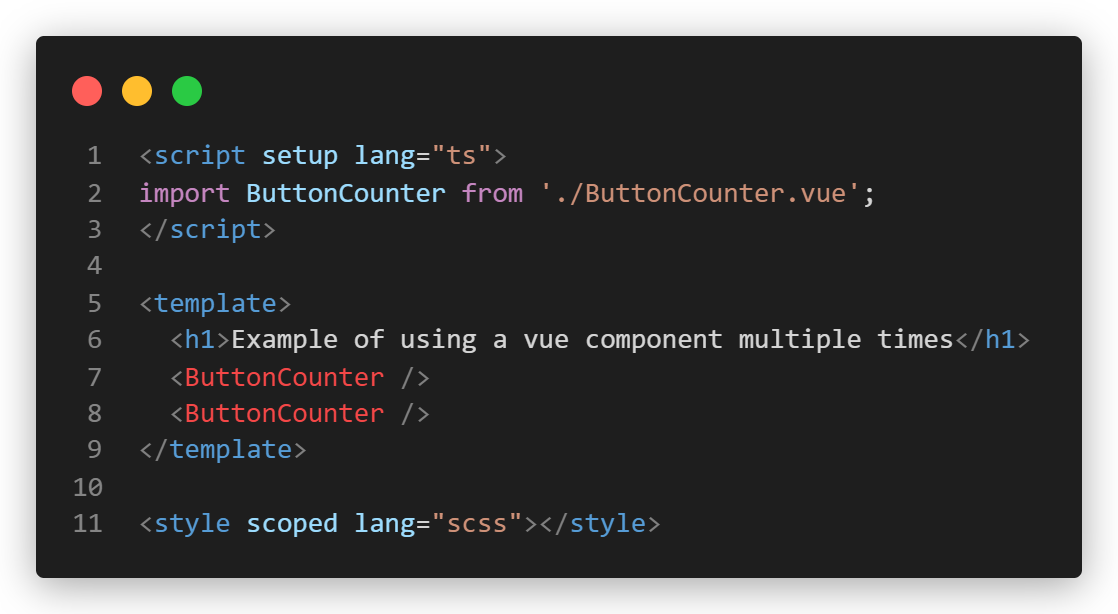
\includegraphics[width=0.9\textwidth]{images/vue-example-usage.png}
  \centering
  \caption[Verwendung einer Vue-Komponente]{Verwendung einer Vue \ac{SFC} \cites[vgl.][]{VueComponentBasics}[vgl.][]{VueSFC}}
  \label{fig:vue-example-usage}
\end{figure}

\textbf{Sprach-Blöcke} \\
In \acp{SFC} können standardmäßig die drei Sprach-Blöcke \lstinline{<template>} (HTML), \lstinline{<script>} (JavaScript) und \lstinline{<style>} (CSS) verwendet werden (siehe Abbildung \ref{fig:vue-example}), die den entsprechenden Code der Komponente beinhalten. Mit dem \lstinline{scoped}-Attribut des \lstinline{<style>}-Blocks kann das CSS für die Komponente gekapselt werden, d.h. es wird nur innerhalb der Komponente angewendet \cite[vgl.][]{VueSFC}.

\textbf{TypeScript und Sass} \\
Für die Entwicklung des Frontends sollen TypeScript und Sass verwendet werden, die bereits in Kapitel \ref{sec:typescript} und \ref{sec:sass} erläutert wurden. So soll sichergestellt werden, dass Fehler bereits während der Entwickler behoben werden können und ein robustes, wartbares Frontend entsteht.

Um TypeScript in einer \ac{SFC} verwenden zu können, muss der \lstinline{<script>}-Block (siehe Abbildung \ref{fig:vue-example}) um das Attribut \lstinline{lang="ts"} erweitert werden. Sass kann nach der Erweiterung des \lstinline{<style>}-Blocks um das Attribut \lstinline{lang="scss"} verwendet werden \cite[vgl.][]{VueSFC}.

%
% Vue - Composition API
%
\subsection{Composition API}
Vue-Komponenten können (innerhalb des \lstinline{<script>}-Blocks) entweder mit Vue's Options API oder mit der Composition API erstellt werden. Aufgrund der Empfehlung von Vue wird im Rahmen dieser Studienarbeit die Composition API in Verbindung mit \acp{SFC} verwendet. Des Weiteren wird das \lstinline{setup}-Attribut des \lstinline{<script>}-Blocks ergänzt (siehe Abbildung \ref{fig:vue-example}), wodurch der Umgang mit der Composition API erleichtert wird. Unter Anderem werden alle Imports sowie Variablen für den \lstinline{<template>}-Block bereitgestellt \cite[vgl.][]{VueIntroduction}.

In Abbildung \ref{fig:vue-example} wird bereits die Composition API verwendet. Im Vergleich dazu zeigt Abbildung \ref{fig:vue-example-options-api} dieselbe Komponente unter Verwendung der Options API.

\begin{figure}[!htb]
  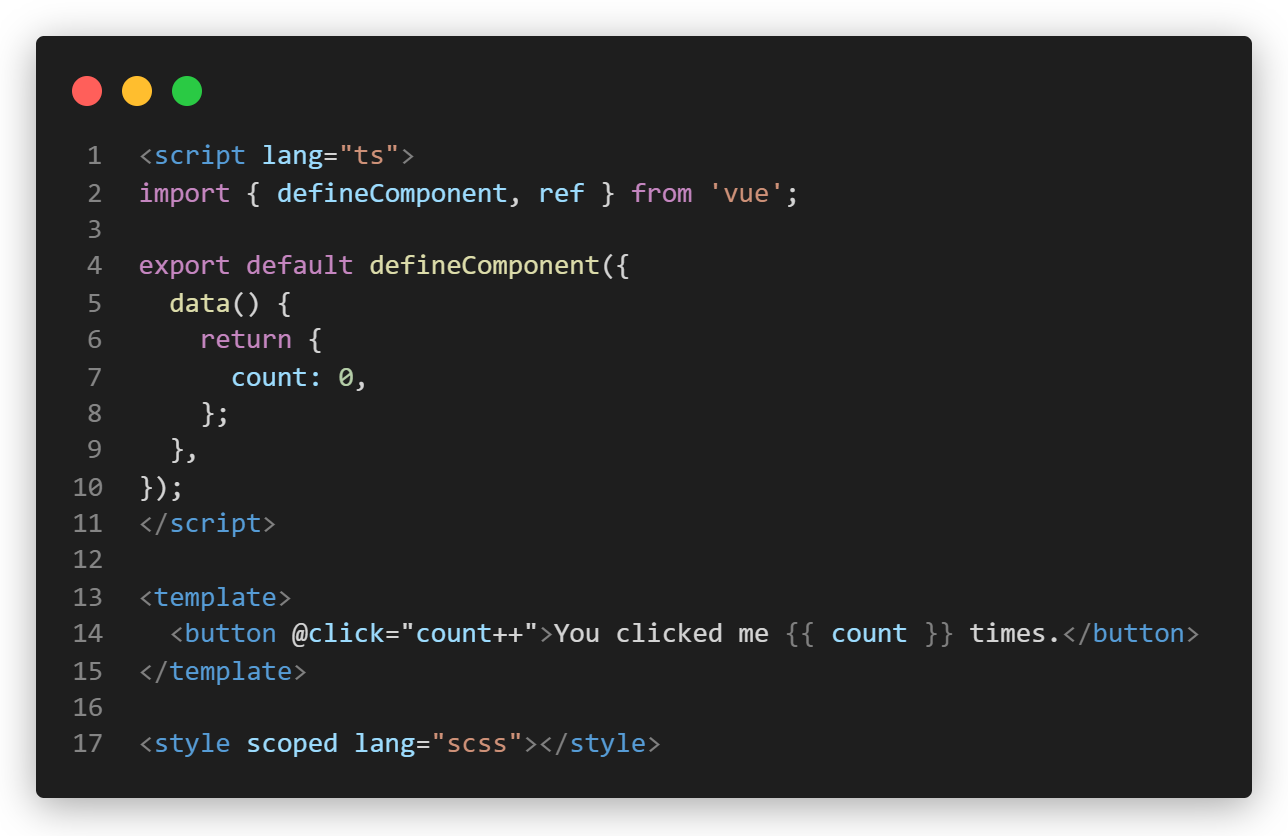
\includegraphics[width=0.9\textwidth]{images/vue-example-options-api.png}
  \centering
  \caption[Beispiel einer Vue-Komponente mit Options API]{Beispiel einer Vue-Komponente mit Options API \cites[vgl.][]{VueIntroduction}[vgl.][]{VueSFC}}
  \label{fig:vue-example-options-api}
\end{figure}

%
% Strapi CMS
%
\section{Strapi CMS}

%
% Heroku
%
\section{Heroku}

\chapter{Projektstruktur}

%
% Frontend
%
\section{Frontend}
Das Frontend besteht aus insgesamt vier Seiten, die im Folgenden näher betrachtet werden sollen. Dabei wird lediglich auf die Seiten als Ganzes und nicht auf jede individuelle Komponente eingegangen. Es sei angemerkt, dass im aktuellen Entwicklungsstand der Studienarbeit Platzhalter für Texte, Bilder etc. verwendet werden, da konkrete Inhalte noch nicht feststehen.

%
% Frontend - Startseite
%
\subsection{Startseite}

Abbildung \ref{fig:frontend-homepage-1} und \ref{fig:frontend-homepage-2} zeigen die Startseite des Frontends. Am Anfang der Seite befindet sich ein großflächiges Bild, das die Aufmerksamkeit des Nutzers anziehen soll. Im Folgenden werden dann die Angebote beschrieben, die die Pflegeeinrichtung anbietet sowie Zitate von Erfahrungsberichten dargestellt. Am Ende der Seite befinden sich Bilder und Daten zum Team und Partner der Pflegeeinrichtung, wodurch eine persönliche Bindung zum Besucher hergestellt werden soll.

\begin{figure}[H]
  \setlength{\fboxsep}{0pt}
  \setlength{\fboxrule}{0.5pt}
  \fbox{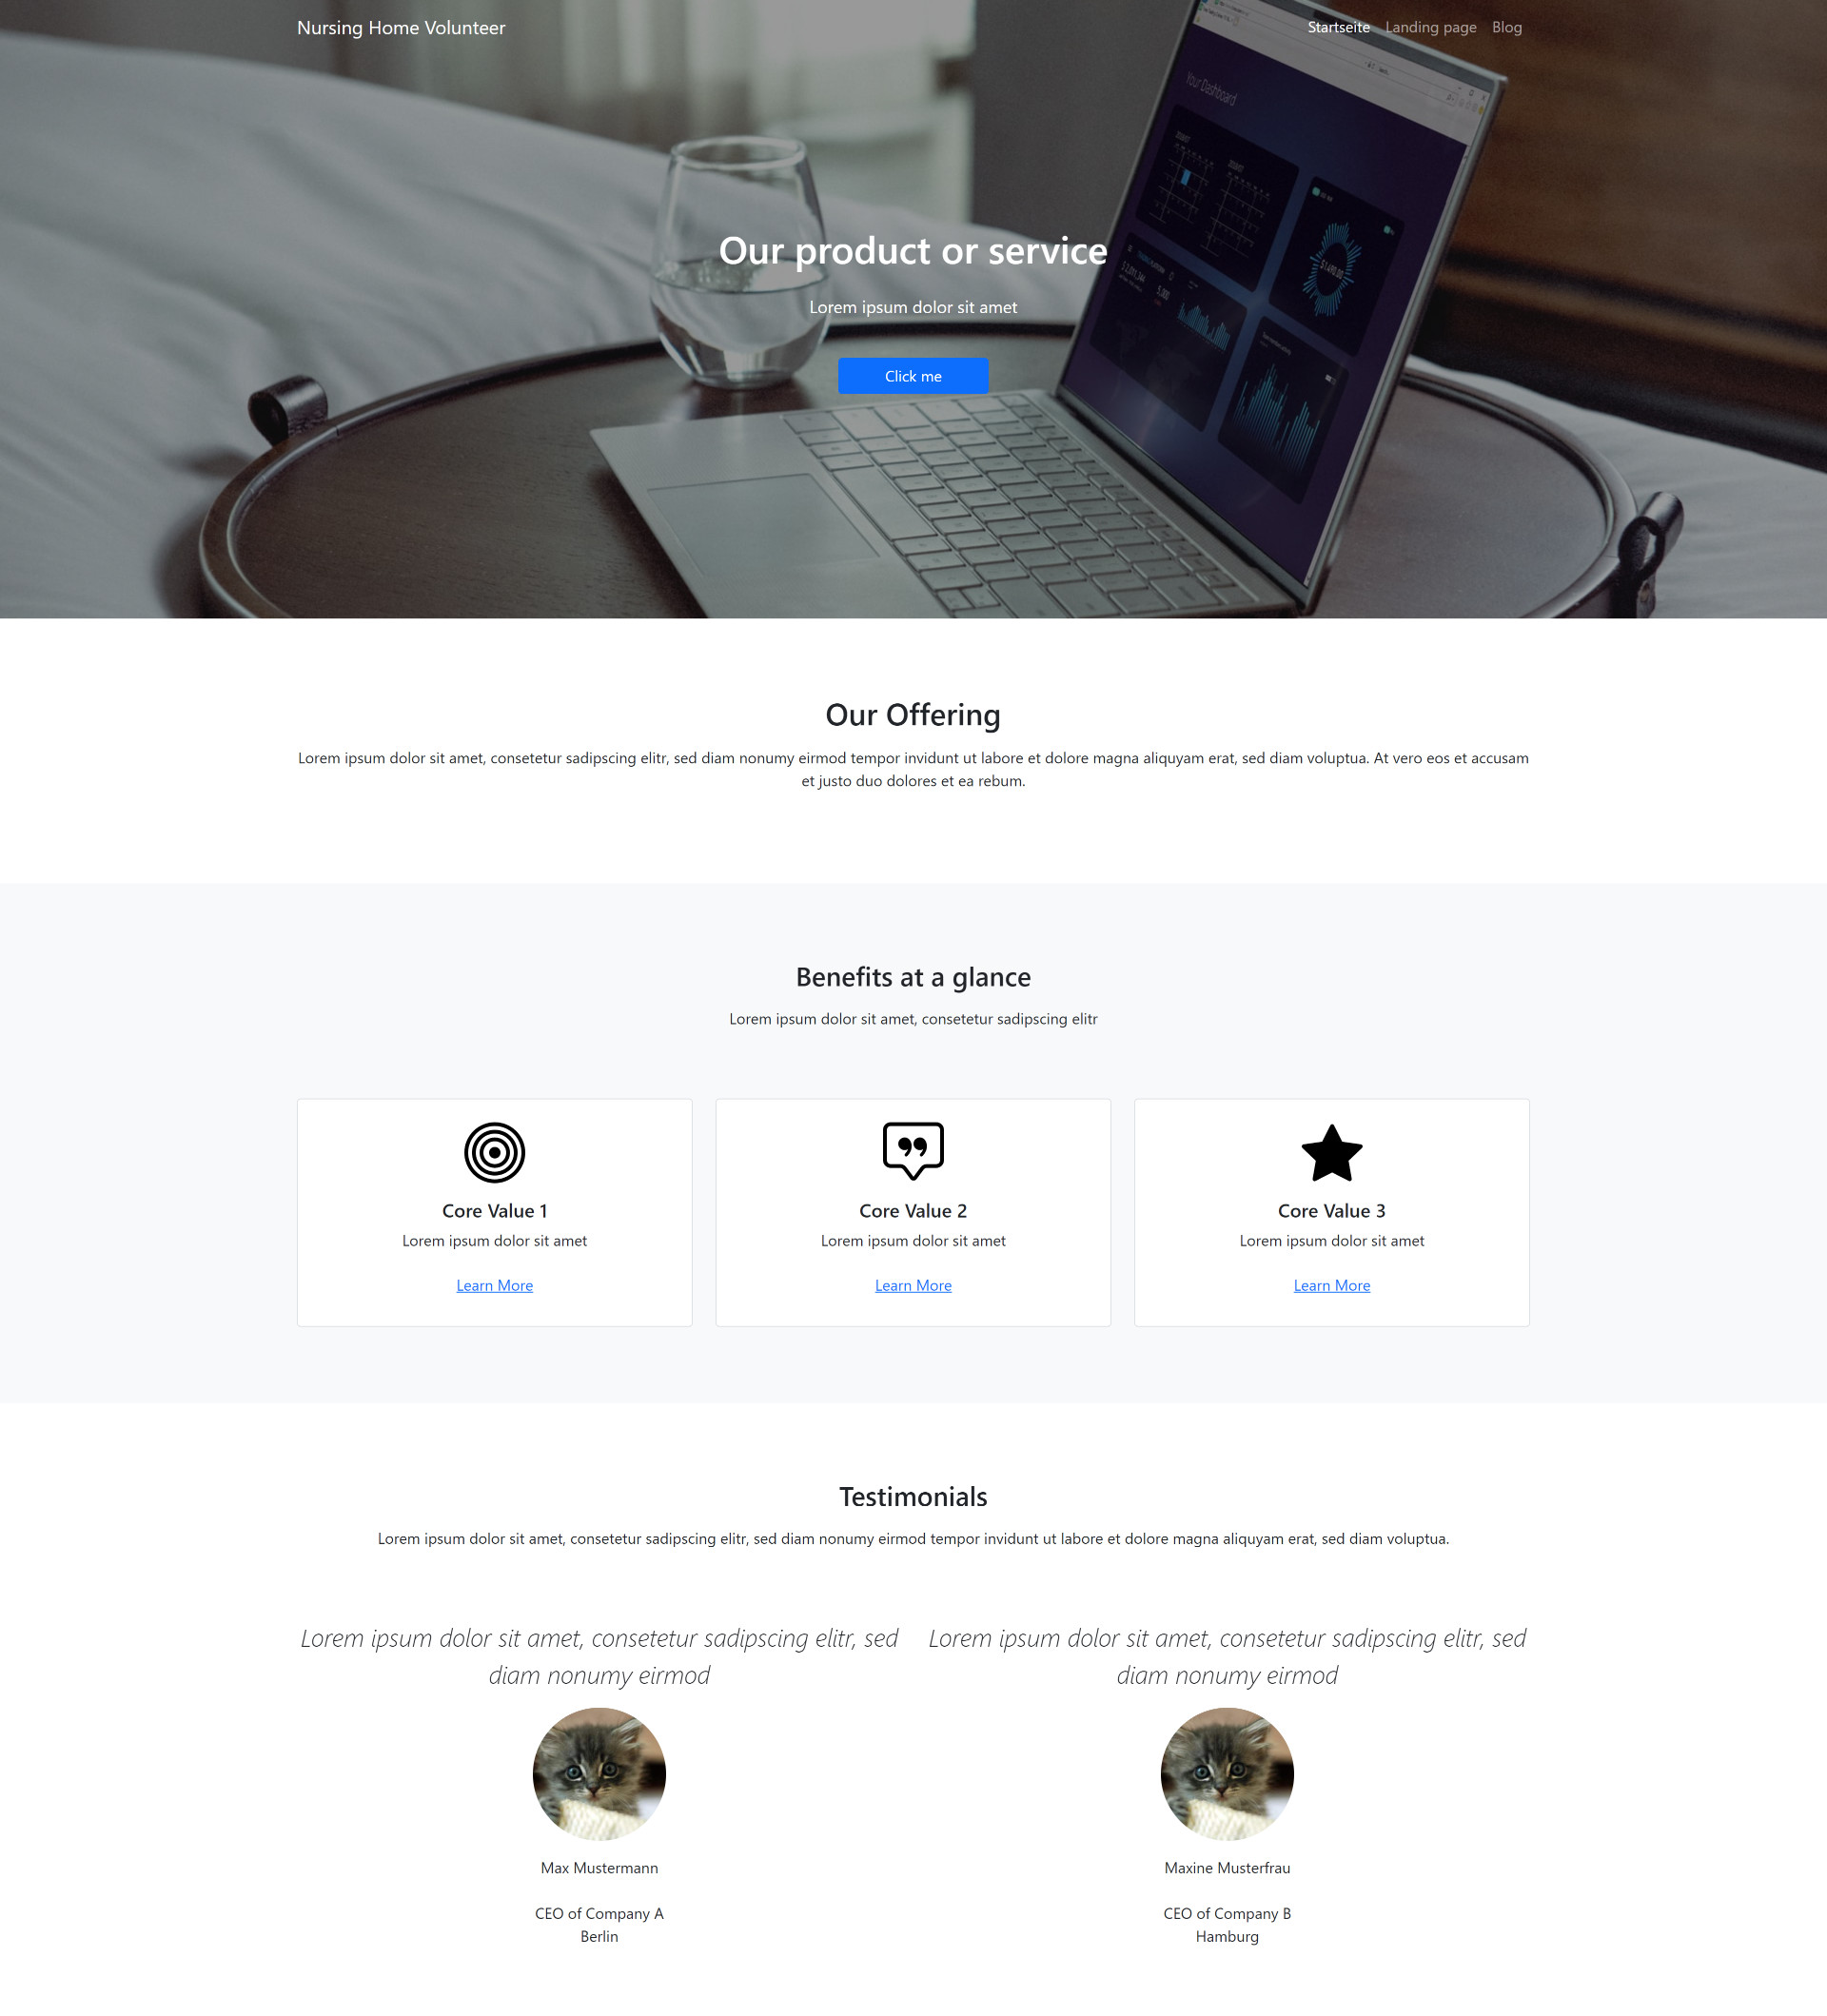
\includegraphics[width=0.9\textwidth]{images/frontend-homepage-1.jpg}}
  \centering
  \caption[Startseite des Frontends Teil 1]{Startseite des Frontends Teil 1}
  \label{fig:frontend-homepage-1}
\end{figure}

\begin{figure}[H]
  \setlength{\fboxsep}{0pt}
  \setlength{\fboxrule}{0.5pt}
  \fbox{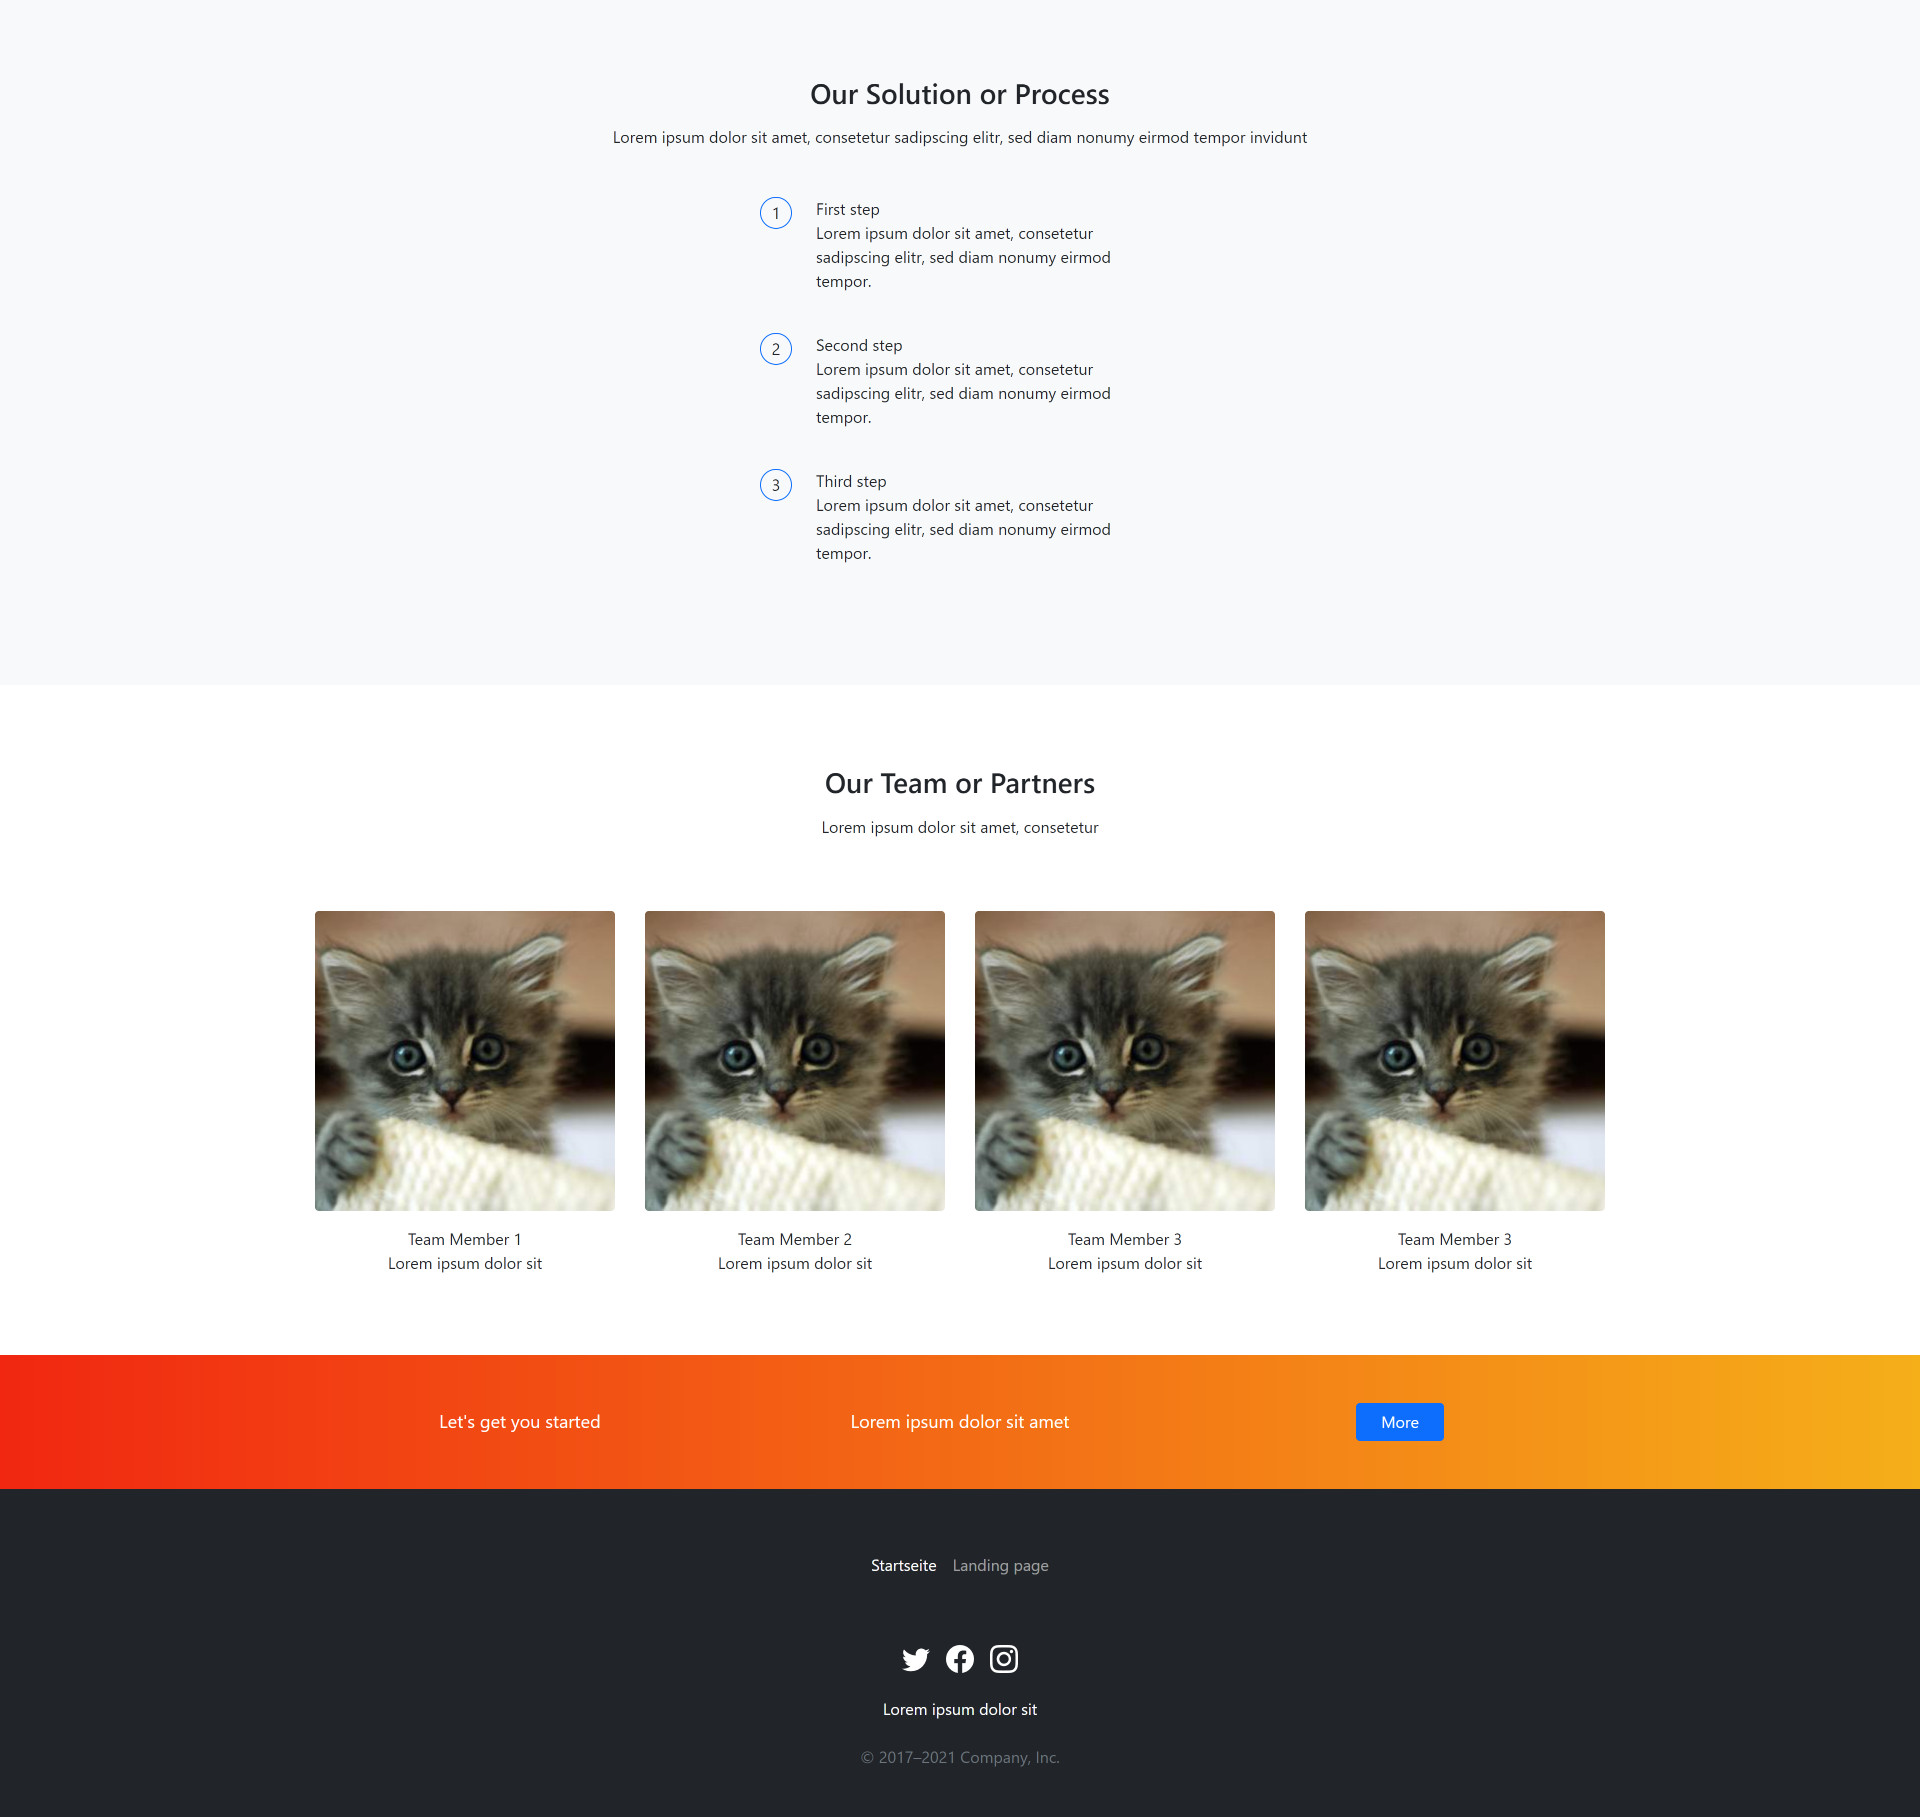
\includegraphics[width=0.9\textwidth]{images/frontend-homepage-2.jpg}}
  \centering
  \caption[Startseite des Frontends Teil 2]{Startseite des Frontends Teil 2}
  \label{fig:frontend-homepage-2}
\end{figure}

%
% Frontend - Landing page
%
\subsection{Landing page}

Die zweite Seite des Frontends ist die sogenannte landing page (siehe Abbildung \ref{fig:frontend-landing-page-1} und \ref{fig:frontend-landing-page-2}), die über die Route \lstinline{/landing-page} erreichbar ist. Diese Seite soll kurz und knapp die wichtigsten Informationen über das Angebot der Pflegeeinrichtung darstellen. Die landing page kann z.B. an Interessierte weitergeleitet werden, um diesen einen vollständigen und kompakten Überblick über alle Angebote zu geben. Alternativ kann diese Seite als Austausch für die Startseite verwendet werden, sollte dieser Wunsch seitens der Pflegeeinrichtung bestehen.

Hervorzuheben ist der interaktive Kopfbereich der Seite, indem der Besucher durch drei verschiedene Ansichten wechseln kann. In Abbildung \ref{fig:frontend-landing-page-1} ist der Hintergrund zwar lediglich grau, jedoch kann für jede Ansicht ein individuelles Hintergrundbild eingefügt werden, um die Seite ansprechender zu gestalten.

\begin{figure}[H]
  \setlength{\fboxsep}{0pt}
  \setlength{\fboxrule}{0.5pt}
  \fbox{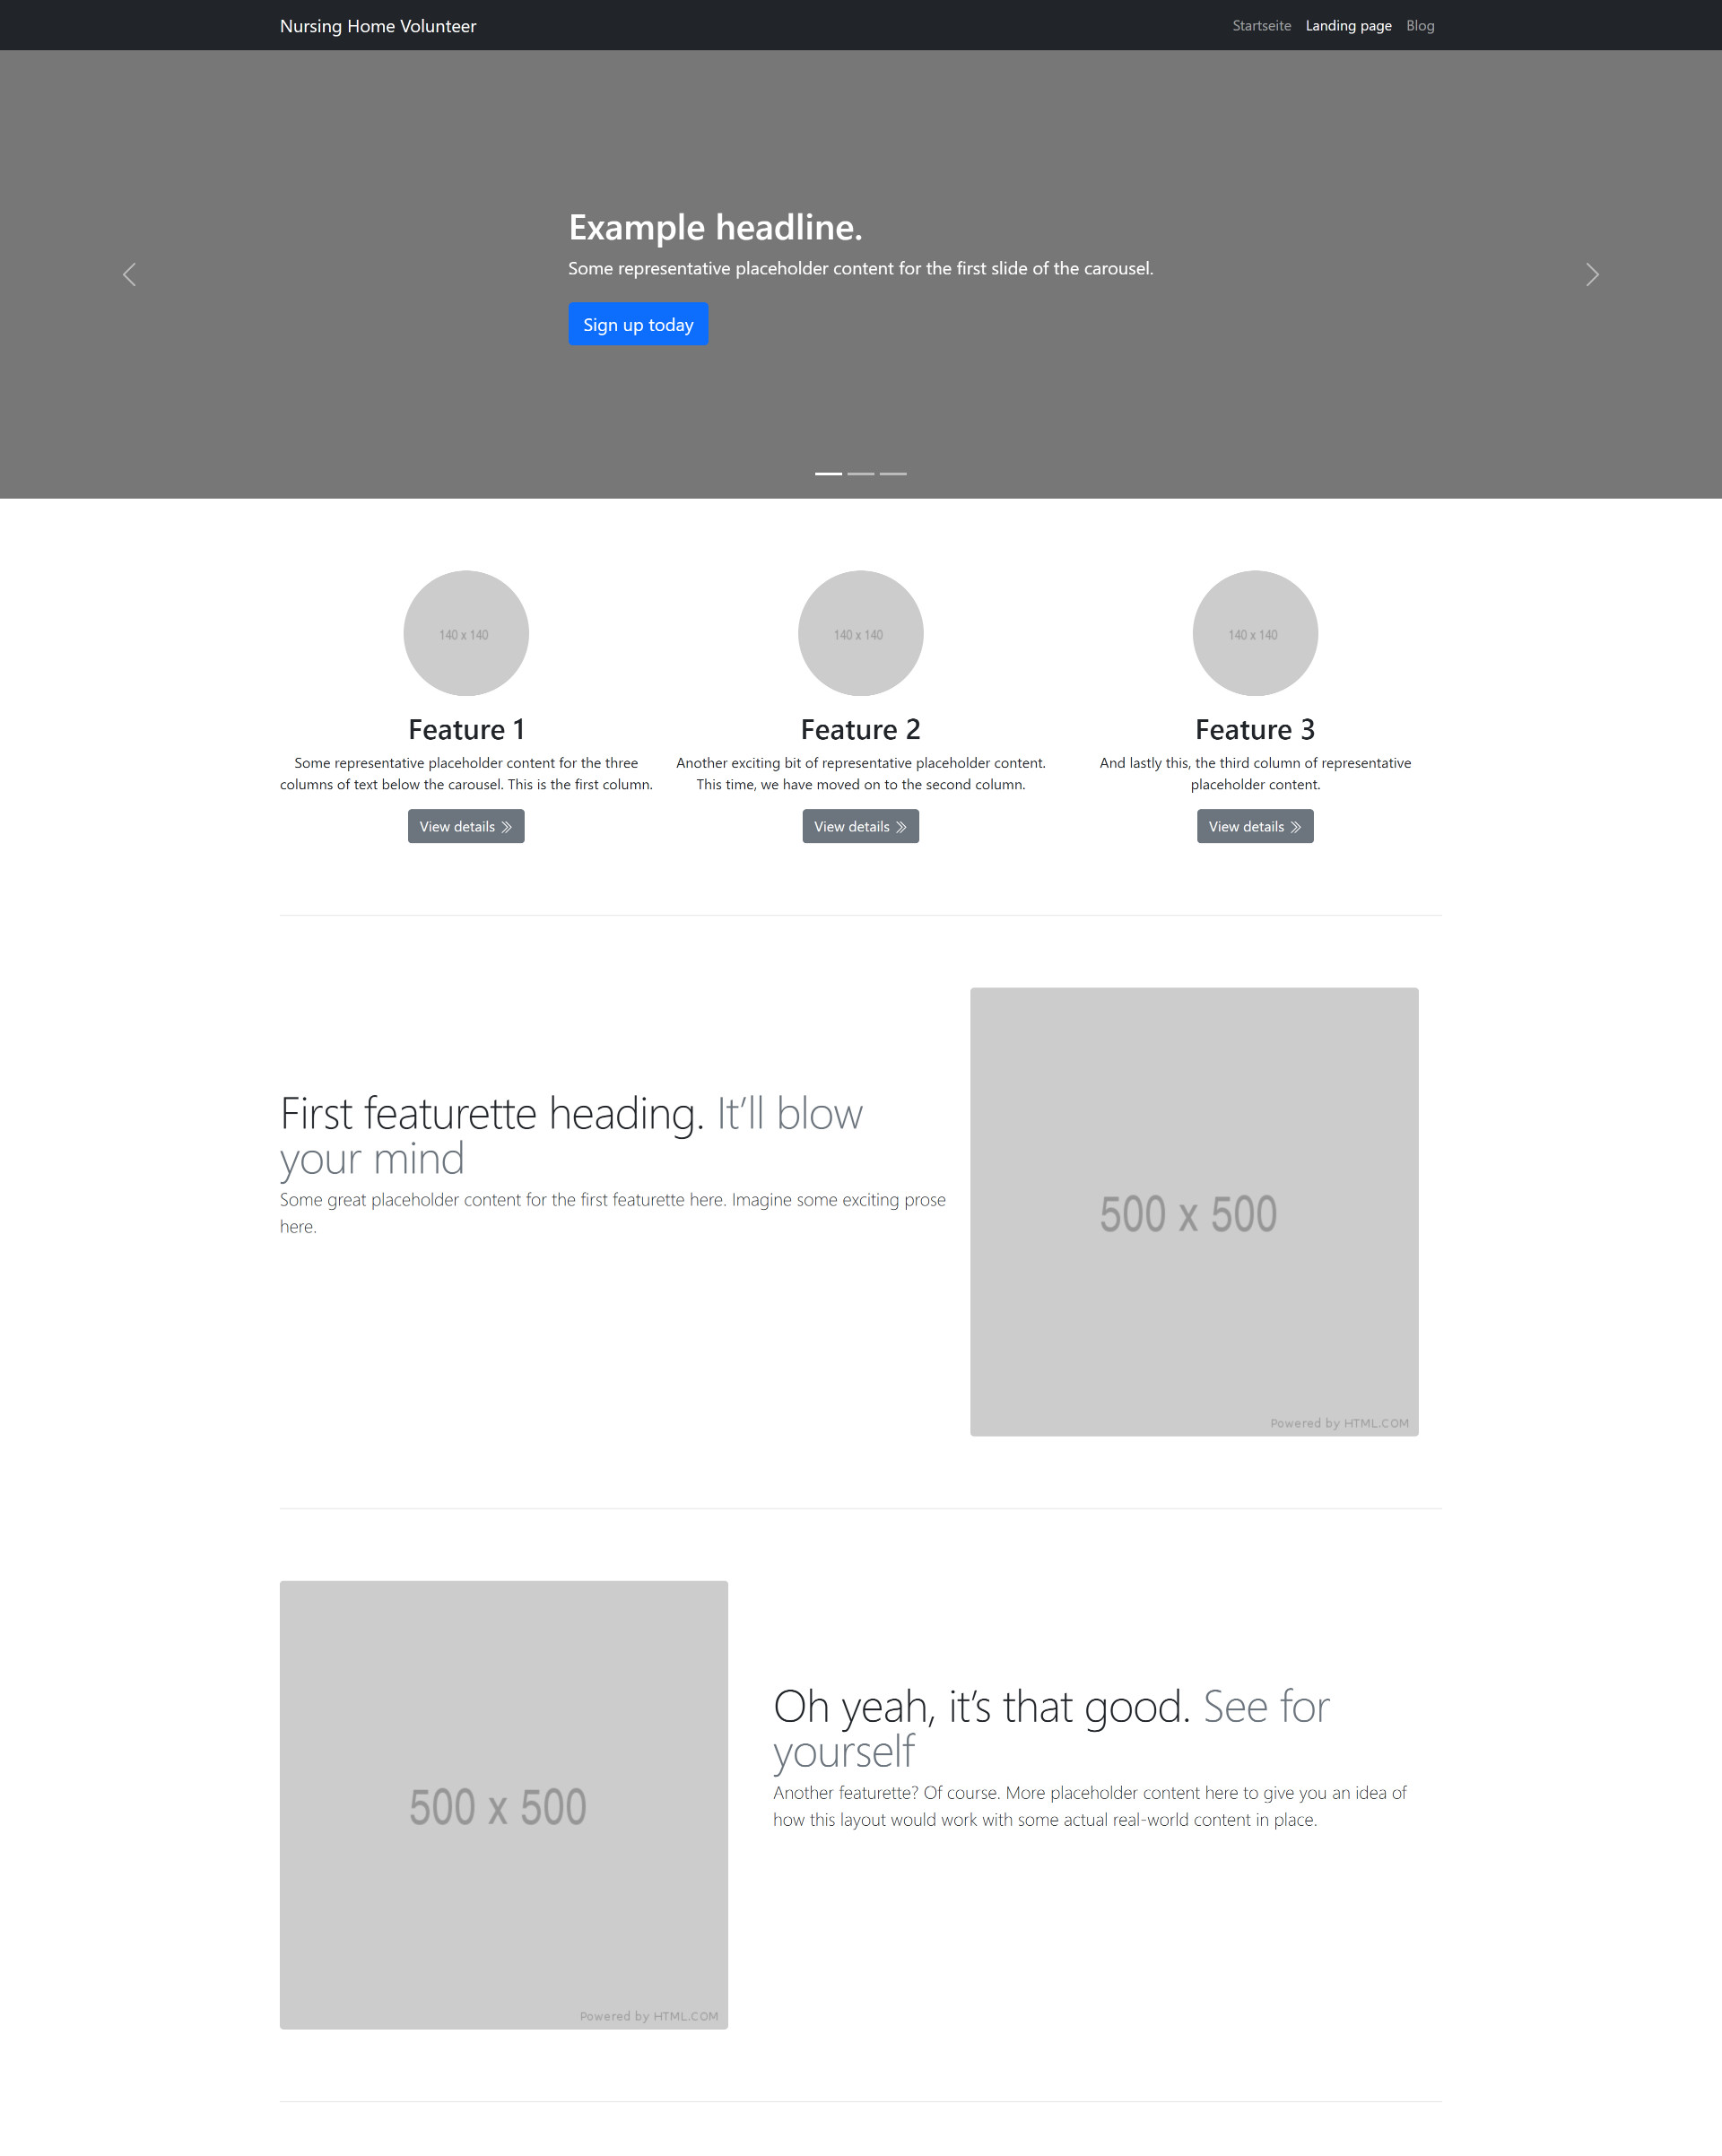
\includegraphics[width=0.85\textwidth]{images/frontend-landing-page-1.jpg}}
  \centering
  \caption[Landing page des Frontends Teil 1]{Landing page des Frontends Teil 1}
  \label{fig:frontend-landing-page-1}
\end{figure}

\begin{figure}[H]
  \setlength{\fboxsep}{0pt}
  \setlength{\fboxrule}{0.5pt}
  \fbox{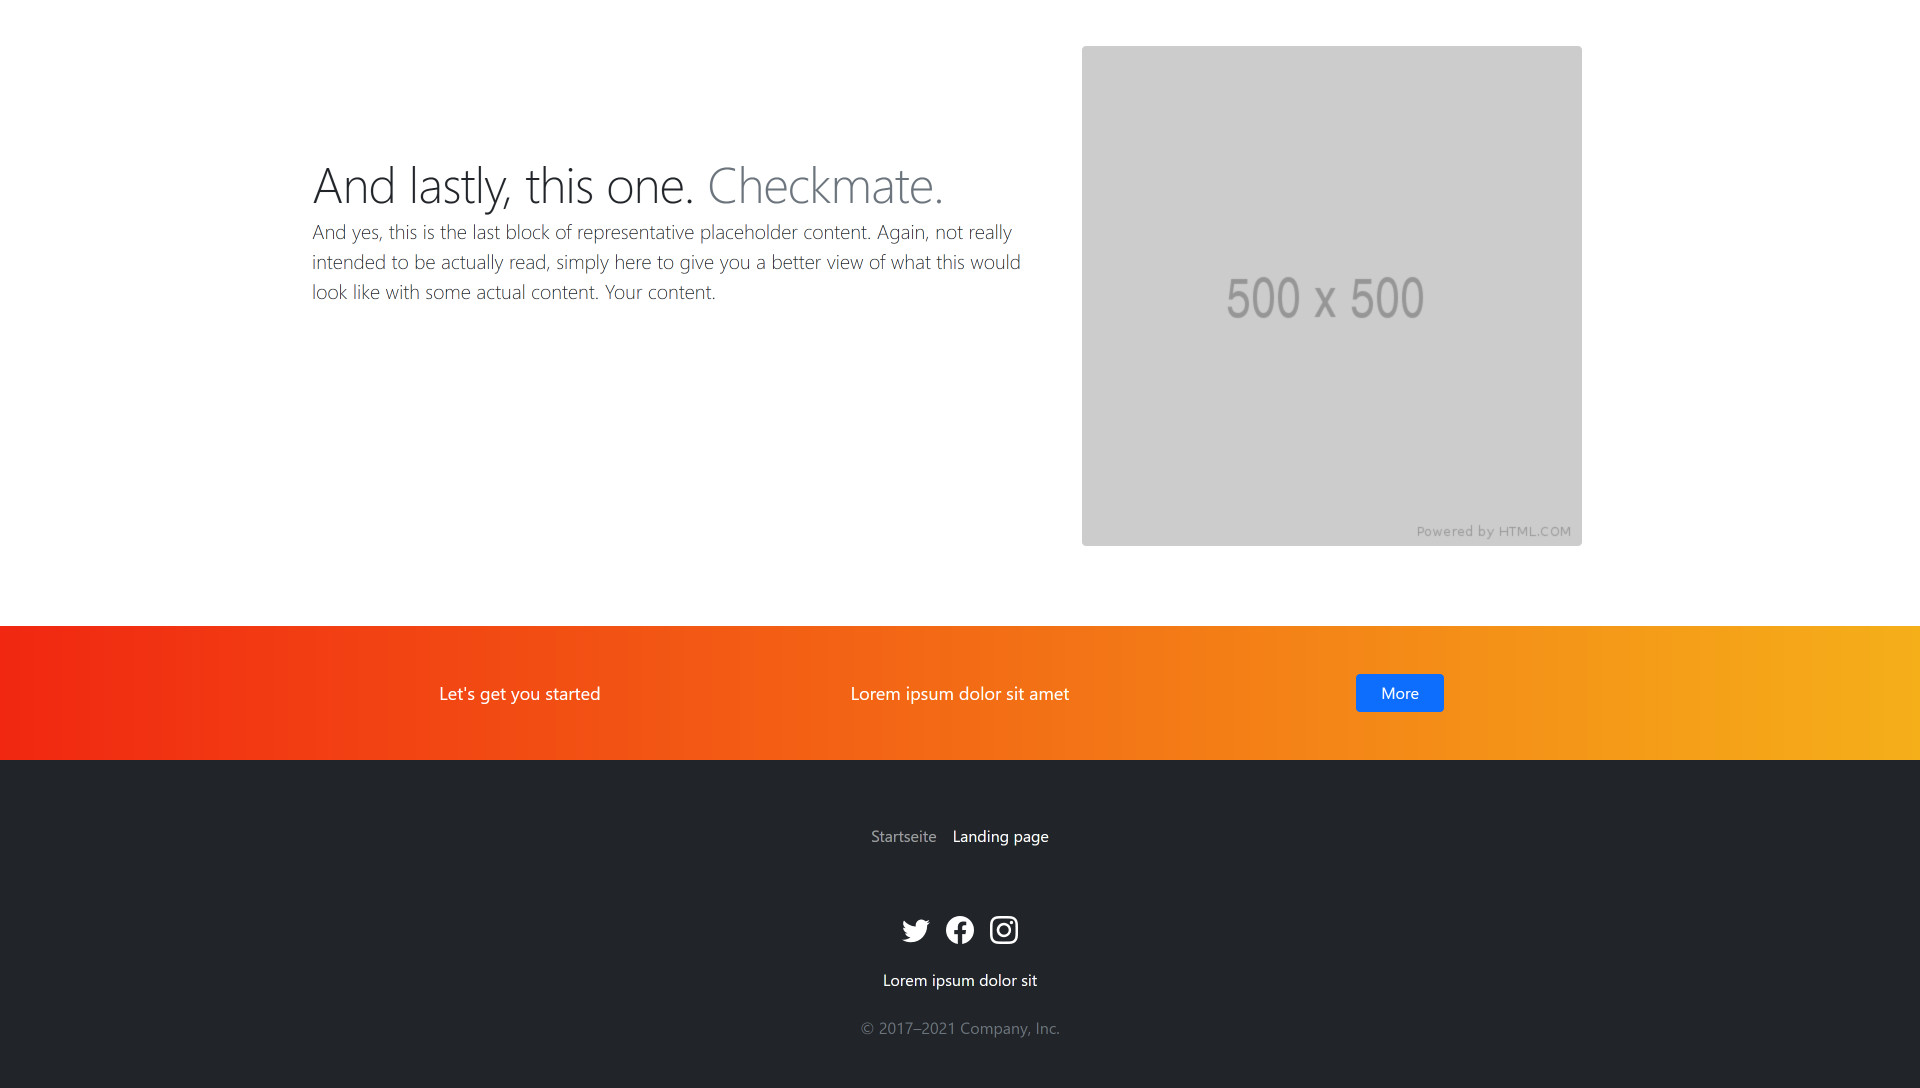
\includegraphics[width=0.9\textwidth]{images/frontend-landing-page-2.jpg}}
  \centering
  \caption[Landing page des Frontends Teil 2]{Landing page des Frontends Teil 2}
  \label{fig:frontend-landing-page-2}
\end{figure}

%
% Frontend - Blog
%
\subsection{Blog}

Der Blog ist die zentrale Stelle für die Ansicht aller Beiträge der Pflegeeinrichtung und ist über die Route \lstinline{/blog} erreichbar. Dabei werden alle verfügbaren Blogbeiträge vom Backend abgerufen und eine Vorschau dieser angezeigt. Ein Klick auf das Bild oder auf die \glqq Weiterlesen\grqq{}-Schaltfläche führt auf die Detailseite des Blogbeitrags.

Links neben den Blogbeiträgen befindet sich ein Platzhalter für Filtermöglichkeiten. Zum aktuellen Entwicklungsstand der Studienarbeit sind die Anforderungen für die Filter seitens der Pflegeeinrichtung noch nicht bekannt. Daher sind diese nicht implementiert.

\begin{figure}[H]
  \setlength{\fboxsep}{0pt}
  \setlength{\fboxrule}{0.5pt}
  \fbox{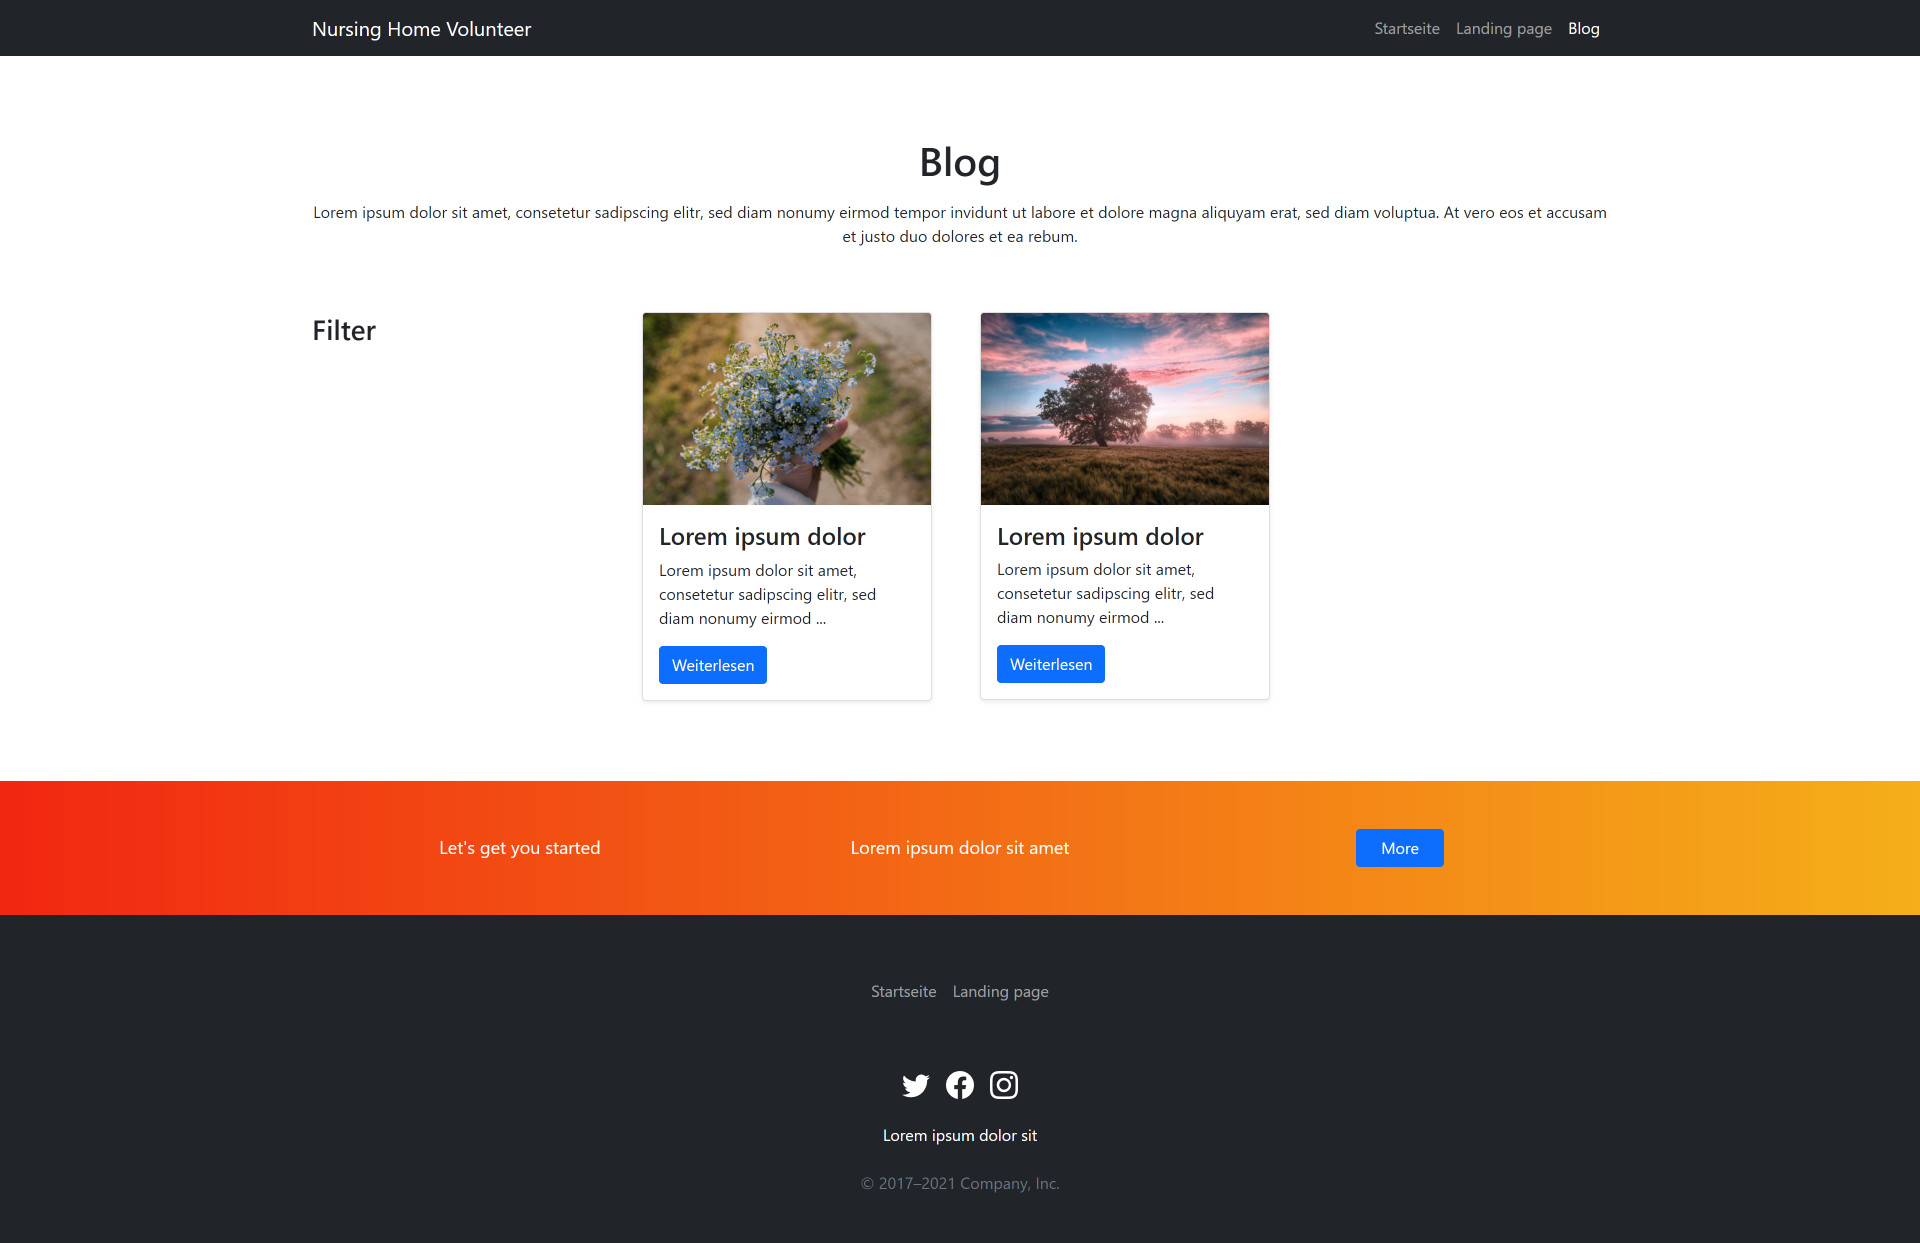
\includegraphics[width=0.9\textwidth]{images/frontend-blog.jpg}}
  \centering
  \caption[Blog des Frontends]{Blog des Frontends}
  \label{fig:frontend-blog}
\end{figure}

%
% Frontend - Blogbeitrag
%
\subsection{Blogbeitrag}

Nach dem Öffnen eines Beitrags im Blog oder durch manuellen Aufruf der URL, gelangt der Besucher auf die Detailseite für einen Blogbeitrag (siehe Abbildung \ref{fig:frontend-blogbeitrag}). Jeder Beitrag ist über die Route \lstinline{/blog/<id>} erreichbar, wobei \lstinline{<id>} durch die eindeutige ID des Beitrags ersetzt werden muss. Beim Aufruf der Seite wird der Blogbeitrag vom Backend abgerufen, falls dieser nicht bereits geladen wurde.

Ein Blogbeitrag besteht aus insgesamt vier Komponenten: Titel, Bild (optional), Beschreibung und beliebig vielen Medienbereichen.

Die Medienbereiche sind, wie in Abbildung \ref{fig:frontend-blogbeitrag} zu sehen, voneinander getrennte Abschnitte, die mindestens eine Beschreibung bzw. Text beinhalten. Der Titel sowie das Medium sind optional. Diese Bereiche können dazu verwendet werden, um den Blogbeitrag inhaltlich zu gliedern sowie mit weiteren Medien zu erweitern. Mögliche Medientypen sind Bilder, Videos, Audiodateien sowie sonstige Dateien (PDFs, Textdateien etc.).

\begin{figure}[H]
  \setlength{\fboxsep}{0pt}
  \setlength{\fboxrule}{0.5pt}
  \fbox{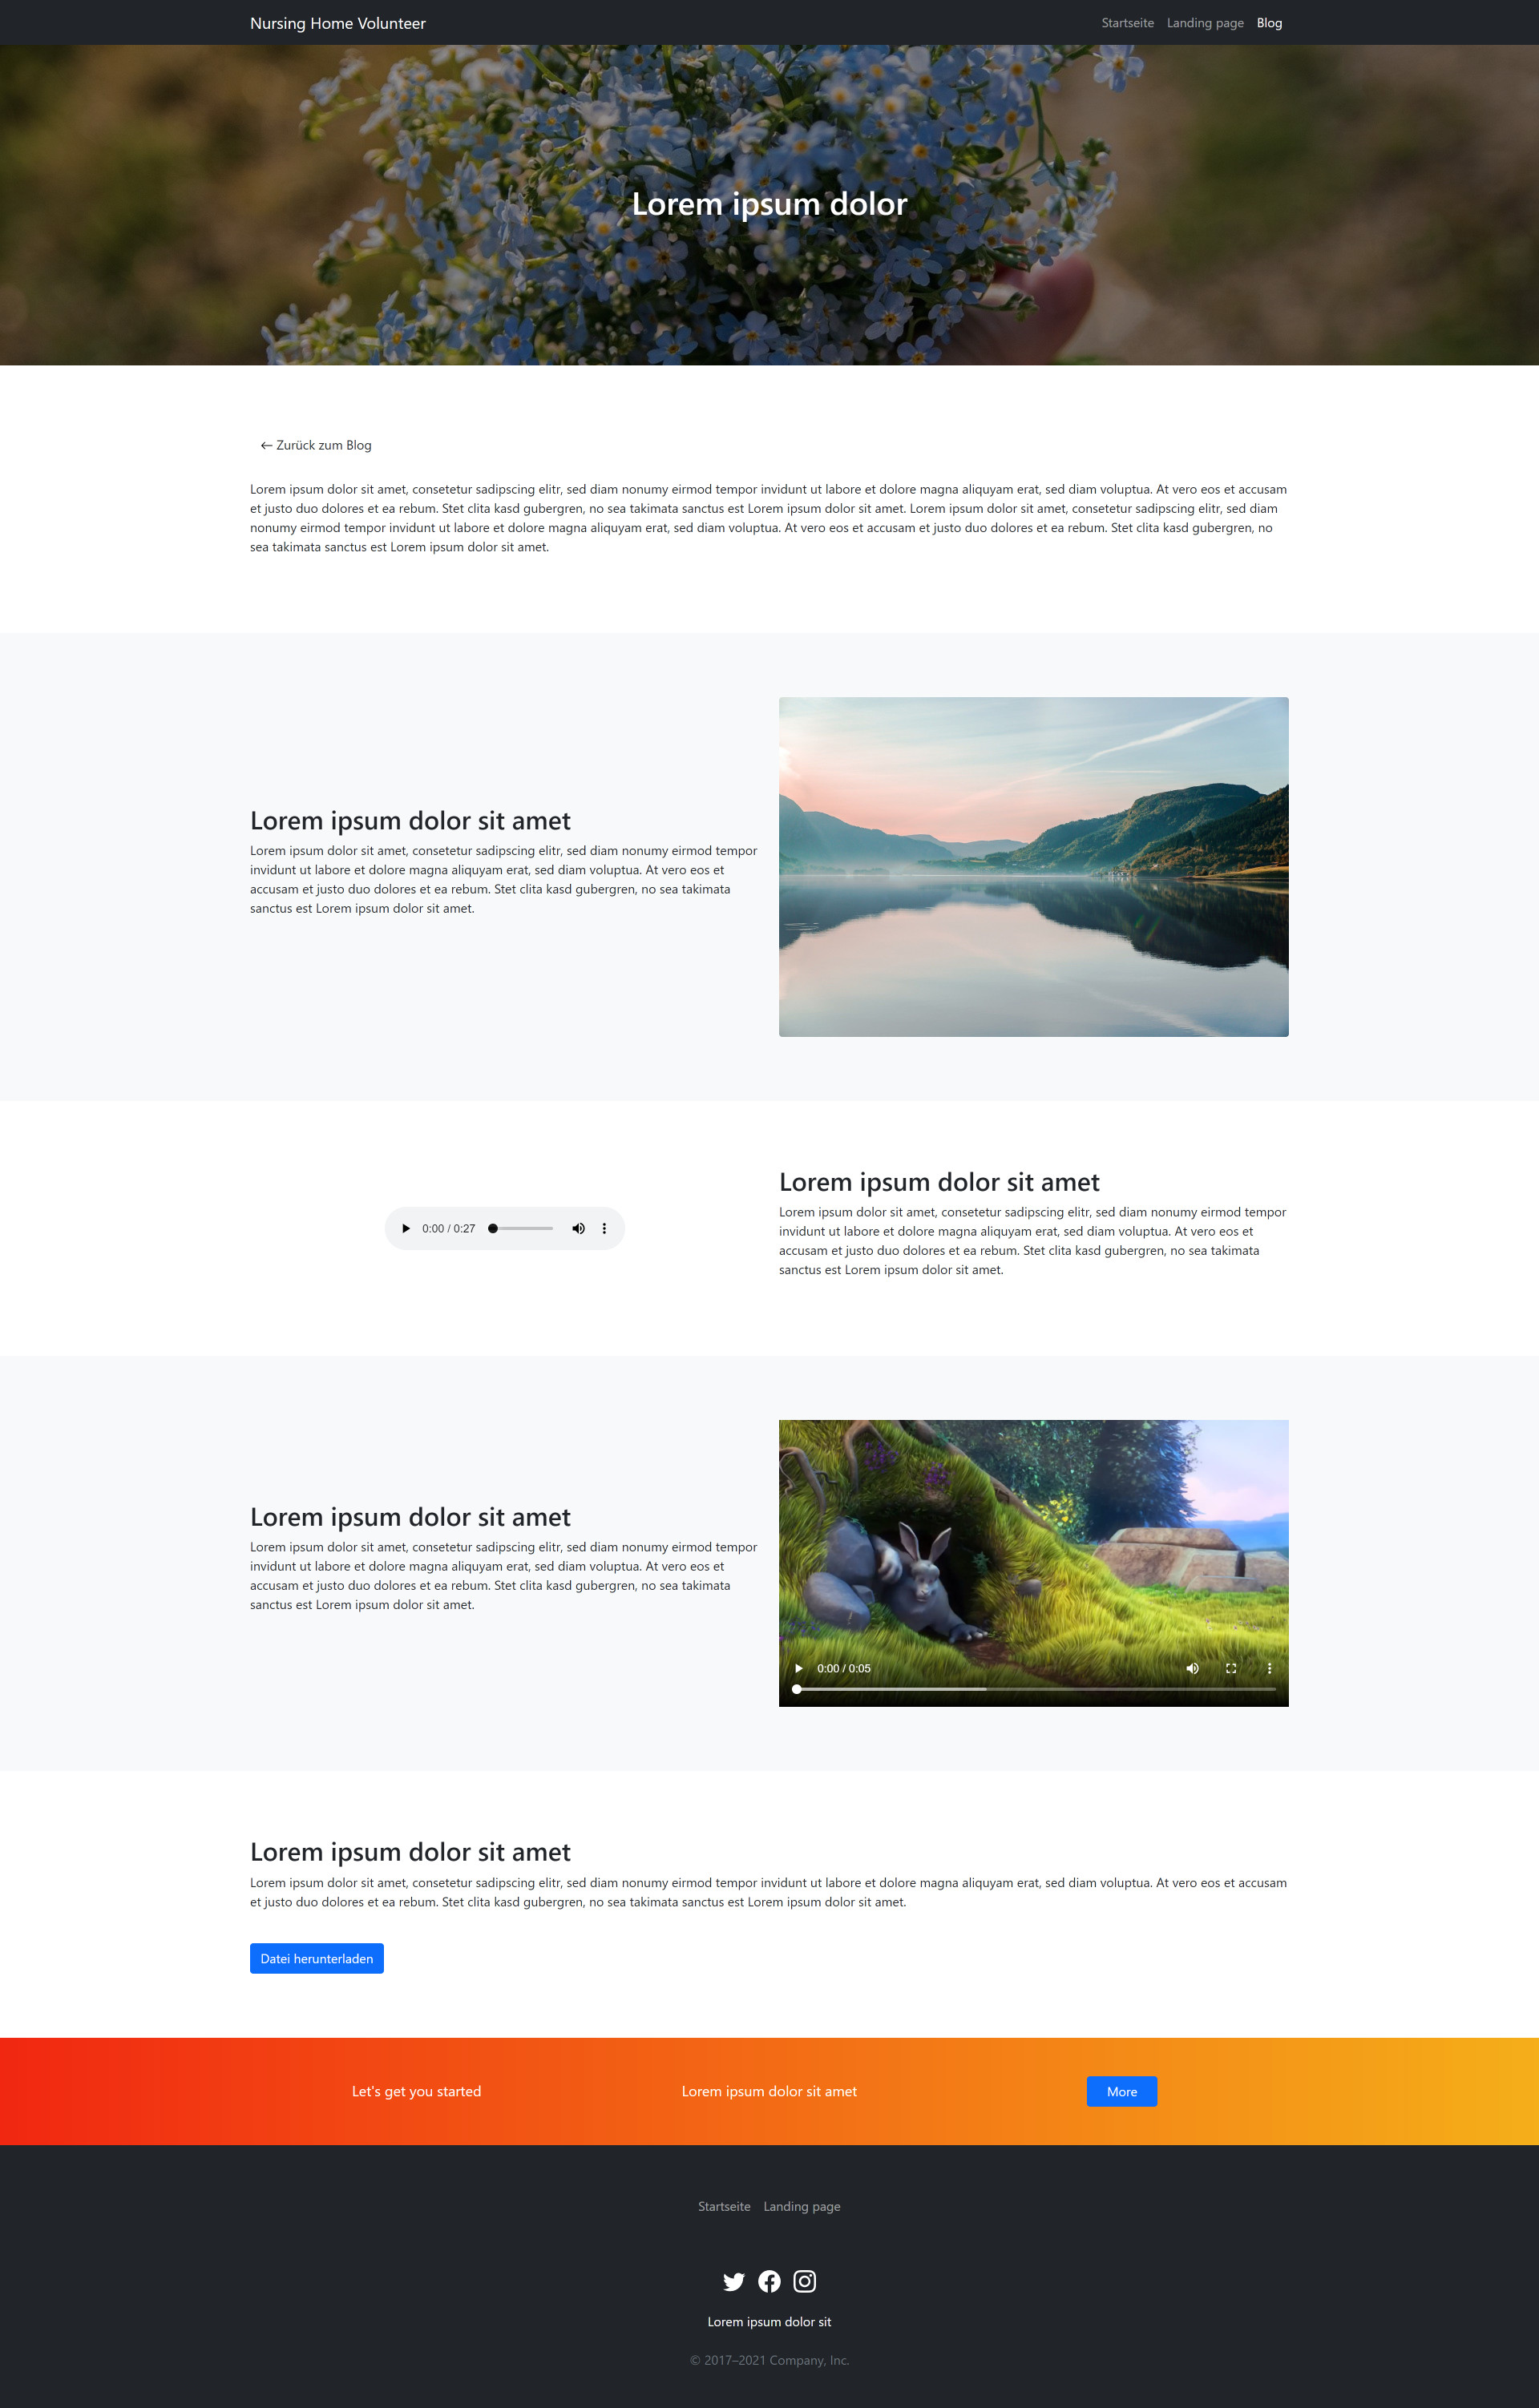
\includegraphics[width=0.85\textwidth]{images/frontend-blogbeitrag.jpg}}
  \centering
  \caption[Blogbeitrag des Frontends]{Blogbeitrag des Frontends}
  \label{fig:frontend-blogbeitrag}
\end{figure}

%
% Frontend - Code-Struktur
%
\subsection{Code-Struktur}

%
% Frontend - Lokale Entwicklung
%
\subsection{Lokale Entwicklung}

\section{Backend}
\label{sec:struktur-backend}

\input{content/fazit.tex}

\backmatter
\sloppy
\printbibliography
\addcontentsline{toc}{chapter}{Literaturverzeichnis}

\pagenumbering{gobble}
\appendix

\part{Datenträger CD}


\end{document}
